%cSpell: ignore usize lgraphs graphviz mygraph Tpng

\chapter{Реализация библиотеки для работы с L-графами}

Для работы с L-графами, была написана библиотека на языке Rust. 
Rust -- современный, высокопроизводительный и безопасный язык, библиотеки которого
можно подключить к другим языкам, или, благодаря поддержки технологии WebAssembly, использовать
в браузере. Вместе с компилятором поставляется программа Cargo -- сборщик проектов (build tool) и менеджер
зависимостей (package manager). 

В библиотеке реализованы ввод-вывод L-графов в текстовом формате, 
алгоритмы построения ядра L-графа, нормальной формы, и проверка достаточных условий регулярности.

Полный исходный код библиотеки можно взять в \cite{github_link}.

\section{Описание структуры библиотеки}

\begin{figure}[h]
    \centering
    \includesvg[scale=0.59, inkscapeformat=png]{images/arch.dot.svg}
    \caption{
        Упрощенная диаграмма классов. Параметр \emph{L} наследует от \emph{Letter}, \emph{N} -- от \emph{Node}, \emph{G} -- от \emph{Graph}.
        Класс \emph{LGraph<G,N,L>} содержит в себе и наследует \emph{Graph<N,LGraphLetter<L>{}>}.
        Синим обозначаются интерфейсы, черным -- классы.
        Черные стрелки -- отношение композиции, зеленые -- наследования.
    }
    \label{arch-image}
\end{figure}

Ключевыми типами в библиотеке являются интерфейс \emph{Graph} и классы \emph{Path}, \emph{DefaultGraph}, \emph{LGraph}, 
поэтому рассмотрим их более детально.

Для реализации \emph{Graph} пользовательскими типами требуется реализовать несколько методов
\begin{itemize}
    \item \emph{nodes()}: метод возвращает итератор по всем вершинам в графе;
    \item \emph{edges()}: метод возвращает итератор по всем дугам в графе;
    \item \emph{start\_node()}: метод возвращает ссылку на начальную вершину графа;
    \item \emph{end\_nodes()}: метод возвращает итератор по всем конечным вершинам графа.
\end{itemize}
Остальные методы имеют реализации по умолчанию, но при желании их можно переопределить.

Класс \emph{Path} описывает пути или маршруты. Он определяется как пустой маршрут, состоящий из одной вершины,
или непустой путь, содержащий список его дуг.
В определении методов \emph{Path} используется одна отличительная черта Rust -- возможность добавлять новые методы для разных 
подстановок типов-аргументов. Это позволяет реализовать методы, связанные только с L-графами, только для
\emph{Path<N, LGraphLetter<T>{}>}.
Еще конкретнее, типы 
\emph{Path<usize, LGraphLetter<char>{}>} и \emph{Path<Memory<usize>, LGraphLetter<char>{}>}
можно считывать из строки и выводить на экран посредством интерфейсов \emph{FromStr} и \emph{Display} из стандартной библиотеки.
Формат строк, описывающих пути, следующий:
\begin{eqnarray*}
    S &\rightarrow& N~|~N~\text{'-'}~E~\text{'->'}~S~|~N~\text{'->'}~S; \\
    E &\rightarrow& char~\text{','}~(\text{'['}~|~\text{']'})~number~|~char~|~(\text{'['}~|~\text{']'})~number; \\
    N &\rightarrow& number; \text{( в случае \emph{usize})} \\
    N &\rightarrow& number~\text{',\{\}'}~|~number~\text{',\{'}~A~\text{'\}'}; \text{( в случае \emph{Memory<usize>})}\\
    A &\rightarrow& number~\text{','}~A~|~number.
\end{eqnarray*} 

\emph{DefaultGraph} является простым примером реализации интерфейса \emph{Graph}.
Он представляет из себя просто список вершин и дуг.
Для \emph{DefaultGraph<usize, LGraphLetter<char>{}>} и \emph{DefaultGraph<Memory<usize>, LGraphLetter<char>{}>}
так же реализованы \emph{FromStr} и \emph{Display}, и граф определяется следующим образом:
\[ S \rightarrow ( N~\text{'->'}~|~\text{'->'}~N~|~N~\text{'-'}~E~\text{'->'}~N~|~N~\text{'->'}~N)~\text{';'}~S.\]

Класс \emph{LGraph<G,N,L>} описывает L-графы, и фактически является просто оберточным типом (wrapper) типа \emph{G},
реализовывающего интерфейс \emph{Graph<N,LGraphLetter<L>{}>}. В этом классе реализованы алгоритмы \emph{core(w, d)}, \emph{normal\_form()},
и методы проверки достаточных условий регулярности. Метод \emph{core(w, d)} возвращает итератор по всем путям из ядра L-графа,
и поэтому поддерживает ленивое выполнение. \emph{LGraph<G,N,L>} так же реализует интерфейсы \emph{FromStr} и \emph{Display},
если конкретный тип \emph{G} их реализует.   
Следует отметить, что этот тип принимает 3 типа-аргумента, однако в Rust реализован механизм type inference, 
во многих случаях позволяющий компилятору из контекста самому понять, какого типа должна быть переменная,
и обычно можно писать просто \emph{LGraph<\_,\_,\_>}. Конечно, в таких случаях, как считывание графа из строки, конкретный
метод реализации этой функции зависит от конкретного типа, и приходится писать полное название типа.

\section{Примеры использования библиотеки}

Для начала, требуется установить Rust. Чтобы создать проект Rust с установленной библиотекой,
можно в терминале прописать следующие команды:

\begin{verbatim}
    $ cargo init lgraphs_example
    $ cd lgraphs_example
    $ cargo add --git https://github.com/0Marble/lgraphs.git graphs
    $ cargo build
\end{verbatim}

\begin{figure}
    \centering
    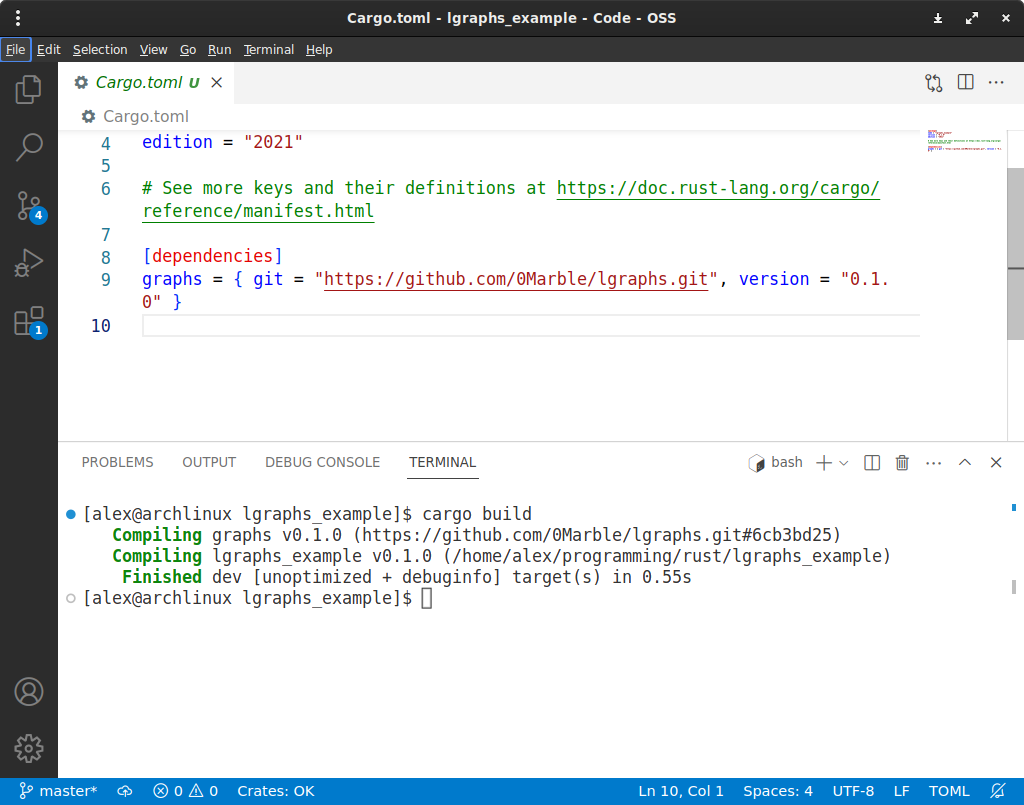
\includegraphics[scale=0.4]{static_images/install_example.png}
    \caption{Проект с подключенной библиотекой}
    \label{project-setup-image}
\end{figure}

Если все прошло успешно, проект должен выглядеть примерно так, как на рисунке \ref{project-setup-image}.
Теперь, в файле \emph{src/main.rs} можно писать собственный код.

Разберем несколько примеров программ.

\subsection{Создание и вывод графа}

\inputminted[linenos]{rust}{../lgraphs/examples/helloworld.rs} \label{helloworld-program}

В строках 6-7 создается переменная типа LGraph \emph{g}, который описывается текстом строки-аргумента
метода \emph{from\_str()}. Метод \emph{from\_str()} может возвращать ошибку, поэтому после него ставится \emph{?}, 
что значит ошибка будет автоматически возвращена вызывающей функцией, в данном случае \emph{main()}.

В строках 9-10 мы выводим L-граф в текстом в консоль двумя способами: первый раз выводим по-умолчанию,
в формате, в котором и вводили граф, второй раз используя формат \emph{DOT} -- известный формат описания графов,
который можно использовать, к примеру, с программой \emph{graphviz} для рисования графов. 

Для запуска программы, воспользуемся командой
\begin{verbatim}
    $ cargo run
\end{verbatim}
Результат работы показан на рисунке \ref{helloworld-out-image}.

\begin{figure}
    \centering
    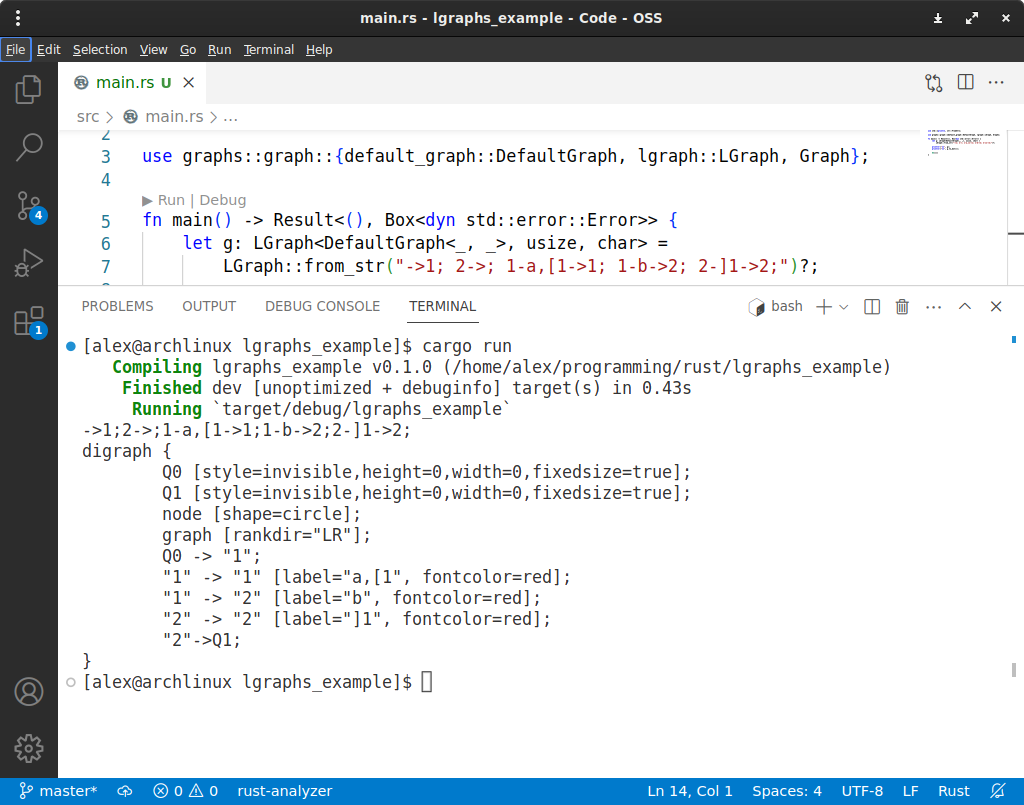
\includegraphics[scale=0.4]{static_images/hello_world.png}
    \caption{Пример запуска программы \ref{helloworld-program}}
    \label{helloworld-out-image}
\end{figure}

\subsection{Вывод ядра L-графа}

\inputminted[linenos]{rust}{../lgraphs/examples/core11.rs} \label{core11-program}

Опять вводим граф \emph{g} из строки. В строке 9, пробегаем по всем пронумерованным индексом \emph{i} путям \emph{t} 
из ядра \emph{Core(g, 1, 1)}, полученным вызовом метода \emph{core(1,1)}. 
Выводим эти строки. Вывод программы в \ref{core11-out-image}.

\begin{figure}
    \centering
    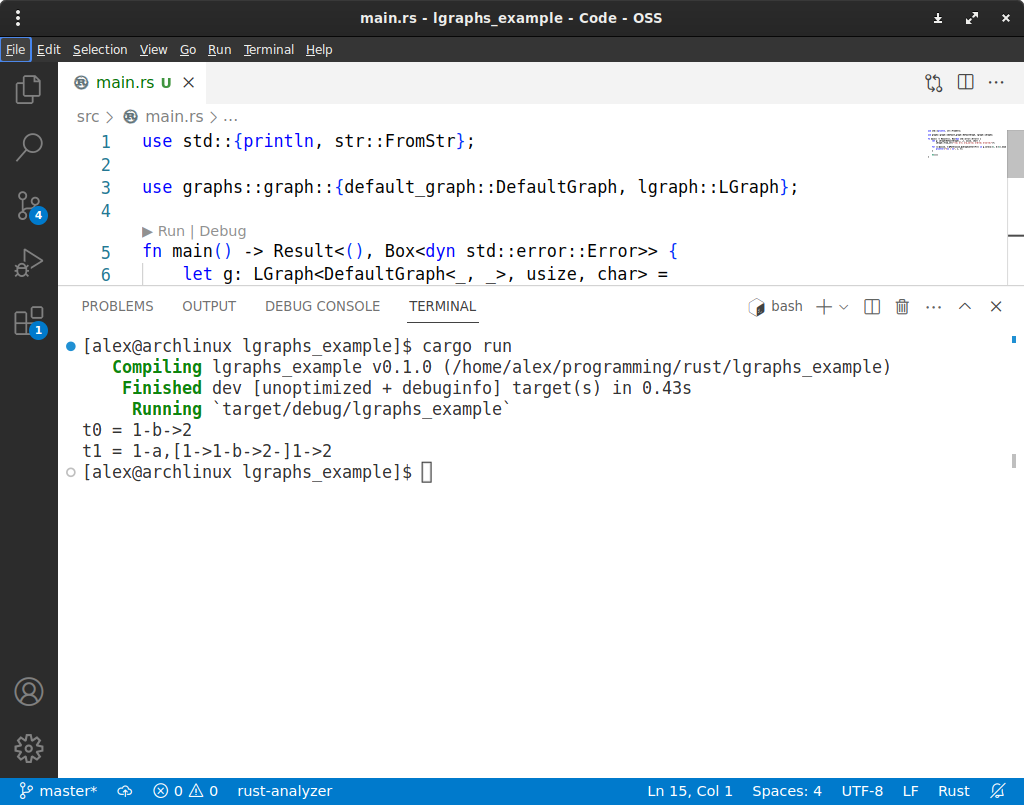
\includegraphics[scale=0.4]{static_images/core11.png}
    \caption{Пример запуска программы \ref{core11-program}}
    \label{core11-out-image}
\end{figure}

\subsection{Проверка регулярности}
\inputminted[linenos]{rust}{../lgraphs/examples/reg.rs} \label{reg-program}

Рассмотрим 3 графа $g1,g2,g3$. Для $g1$ прверим условие \ref{condition_no_letters}, 
для $g2$ условие \ref{condition_no_brackets}, для $g3$ -- \ref{condition_one_sided_loops}.
Результаты проверки выведем на экран, все будут \verb | true |.

\subsection{Построение нормальной формы}
\inputminted[linenos]{rust}{../lgraphs/examples/normal.rs} \label{normal-program}

В этой программе следует отметить, что метод \emph{normal\_form()} требует параметр-тип графа, который является основой
L-графа, поэтому приходится писать \emph{normal\_form::<DefaultGraph<\_, \_>{}>()}.

В этот раз рассмотрим пример интеграции с языком описания графов \emph{DOT}, и сохраним результат как рисунок.
Для этого требуется установить \emph{graphviz}, после чего можно воспользоваться следующей командой:
\begin{verbatim}
    $ cargo run | dot -Tpng > mygraph.png
\end{verbatim}

Вывод нашей программы передастся команде \emph{dot}, которая сгенерирует изображение \emph{mygraph} такого вида,
как на \ref{normal-out-image}.

\begin{figure}[h]
    \centering
    \includesvg[scale=0.7]{static_images/mygraph.svg}
    \caption{Пример запуска программы \ref{normal-program}}
    \label{normal-out-image}
\end{figure}


\pagebreak